\documentclass{article}
\usepackage{graphicx}  % For including images
\usepackage{hyperref}  % For hyperlinks

\title{Eidos: A Tabletop Role-Playing Game}
\author{}
\date{}

\begin{document}

\maketitle

\begin{figure}[h]
    \centering
    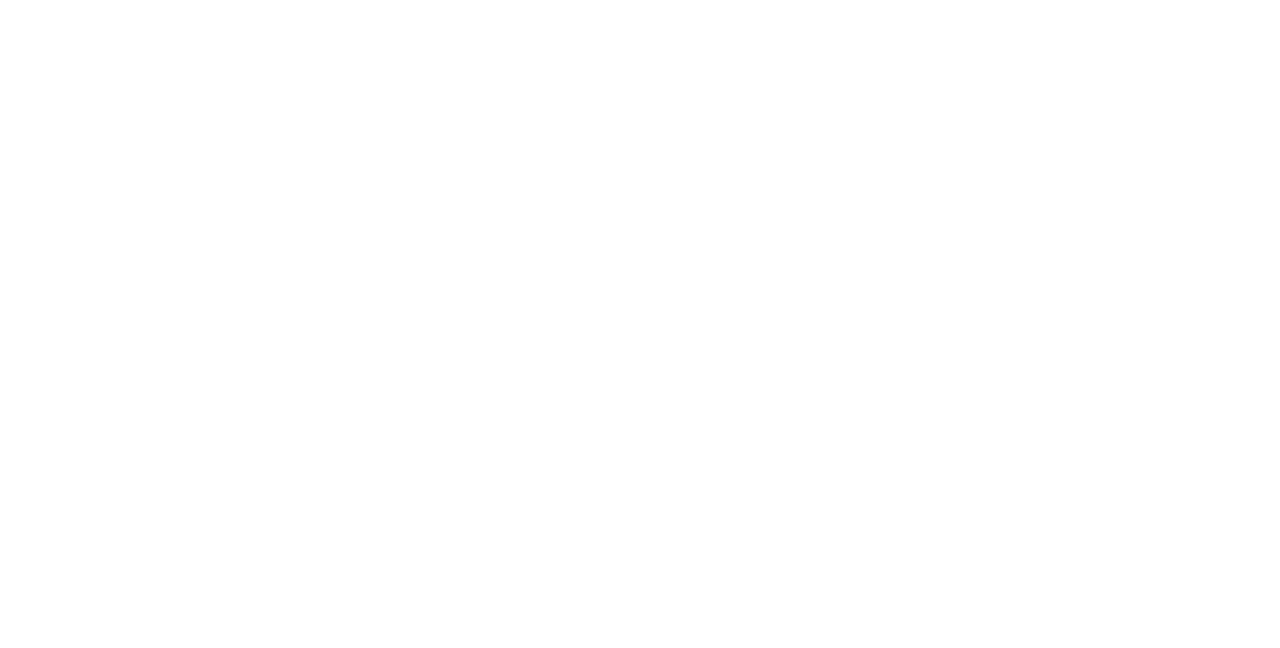
\includegraphics[width=0.7\textwidth]{./images/index01.svg}
    \caption{Eidos Logo}
\end{figure}

\section{Presentation}

In the realm of tabletop role-playing games, \textbf{Eidos} stands as a unique and innovative addition to the genre. Rooted in the principles of open-source development, this game is designed to be both immersive and accessible, offering a deep and rich narrative experience that is driven by player choice. 

Eidos takes its name from the ancient Greek concept of the world of ideas, reflecting the game's focus on immersive and thought-provoking narratives. This name is a nod to the idea that in role-playing games, players have the ability to explore and interact with an imagined world filled with endless possibilities.

The character creation process in \textbf{Eidos} is a deep and engaging experience, allowing players to build their characters from the ground up. With character sheets devoted to personality, religion, physical description, background, clothing, equipment, and skills, players have the tools to create a truly unique and memorable character.

The combat system in \textbf{Eidos} is designed to be immersive and engaging, with mechanics that create dynamic and exciting combat scenes. The game's mechanics are based on classic combat narratives, striving to be a simulation of combat rather than simply a turn-based dice-rolling game. While the standard rules are intended for a pre-modern low-fantasy setting, \textbf{Eidos} is easily adaptable to other role-playing scenarios.

This rulebook is divided into six chapters, each covering a different aspect of the game:

\begin{itemize}
    \item \textbf{Chapter 1: Character Creation} – Provides a detailed guide to creating your character, including sections on personality, religion, physical description, background, clothing, equipment, and skills.
    
    \item \textbf{Chapter 2: Combat and Combat Resolution} – Covers the mechanics of combat in \textbf{Eidos}, including basic combat mechanics, ability checks, skills, tactical maneuvering, environmental interaction, morale, reinforcements, ranged combat, unarmed combat, weapon mechanics, grappling, healing, shields and armor, mounted combat, naval combat, aerial combat, siege weapons, traps, stealth, mass combat, and death and dying.
\end{itemize}

\end{document}
